% !TeX document-id = {7b46d8ca-c04e-4bbc-b88e-52d87e63aa00}
% !TeX TXS-program:compile = txs:///pdflatex/[--shell-escape]
% The commment above is needed to use minted.
\documentclass[11pt]{article}

\usepackage[utf8]{inputenc}

% Limit the page margin to only 1 inch.
\usepackage[a4paper, margin = 1in]{geometry}

% Line spacing
\linespread{1}

% Enable importing external graphic files and provides useful commands, like \graphicspath{}
\usepackage{graphicx}
% Images are located in a directory called "images" in the current directory.
\graphicspath{{./images/}}

\usepackage{amsmath}
\usepackage{amssymb}
\usepackage{bm}
\usepackage{multicol}
% Make links look better by default.
% See: https://tex.stackexchange.com/questions/823/remove-ugly-borders-around-clickable-cross-references-and-hyperlinks
\usepackage[hidelinks]{hyperref}
\usepackage{xcolor}
\hypersetup{
	colorlinks,
	linkcolor={red!50!black},
	citecolor={blue!50!black},
	urlcolor={blue!80!black}
}
\usepackage{minted}
\definecolor{LightGray}{gray}{0.95}
\setminted[python]
{
	frame=lines,
	framesep=2mm,
	bgcolor=LightGray
}

\title{Predicting Apartment Prices in Queens\\
	\vspace{8pt}
	\normalsize Final project for MATH 342W Data Science at Queens College\\
}
\date{}


\begin{document}
	\maketitle
	\begin{center}
		March 25th, 2025
	\end{center}
	\begin{flushright}
		By Sergio E. Garcia Tapia\\
		In collaboration with:\\
		~Paidi Mather~\\
		~Ye Htut Maung~\\
		~Allen Singleton~\\
		~Esther Yee~\\
	\end{flushright}
	\begin{abstract}
		Prediction is both an art and a science with important ramifications
		and applications. It can be used to get ahead of natural disasters
		by predicting aspects of natural disasters, or to earn money by
		exploiting information about the economy. Yet another modest application,
		and the one explored in this paper, is to predict the price of apartments.
		This matters to many, particularly to those who are attempting to attain
		the American dream by purchasing a home rather than a house. In
		this paper, we explore scientific and artistic aspects of data science
		used to make predictions in the context of predicting apartment prices.
	\end{abstract}
	\pagebreak
	\section{Introduction}
	When residents in Queens, NY turn to home ownership, many consider buying
	a house instead of an apartment. Though apartments offer less opportunities
	for renovation and privacy, they can be a more reasonable investment for
	many. At first glance, predicting apartment prices may seem unnecessary
	because apartments that are available for sale tend to list a price.
	However, sellers may withhold the price in hopes that people bid on their
	property, or a buyer may be curious about an apartment with specific
	characteristics that is not currently available for sale. Given historical
	information about apartment listings, we can build a predictive model
	that can be of use in these situations.
	
	A predictive model is a function used to make approximations about
	a phenomenon of interest using some given data. In this context,
	we are approximating the sale price of apartments in Queens, NY.
	More concretely, a predictive model is designed to answer the question:
	given a unit of observation represents an apartment, with a set of
	features including but not limited to number of bedrooms and bathrooms,
	location, and whether cats are allowed, what is its sale price?
	Using the same historical data, we will apply a variety of modeling approaches,
	namely a regression tree model, a linear model, and a random forests model.
	We will explore the trade-offs made by these models, mainly in account of
	interpretation and predictive performance.
	\section{The Data}
	The data set used in this project consists of 2230 observations obtained
	from MLSLI via Amazon Mturk. Each observation has 55 columns, of which about 28
	include only metadata information related to Mturk, but is otherwise unrelated
	to the entries. Each observation corresponds to an
	apartment listing that was available for sale between February 2016 and 2017,
	with information such as: whether pets are allowed, the year the apartment was
	built, the number of rooms, and the kitchen type, among others. Unfortunately,
	2230 is not a large enough sample to build a strong model for predicting
	apartment prices in Queens, considering that there are millions of units in NYC.
	Thus, the models we build are not expected to extrapolate well.
	\begin{figure}
		\centering
		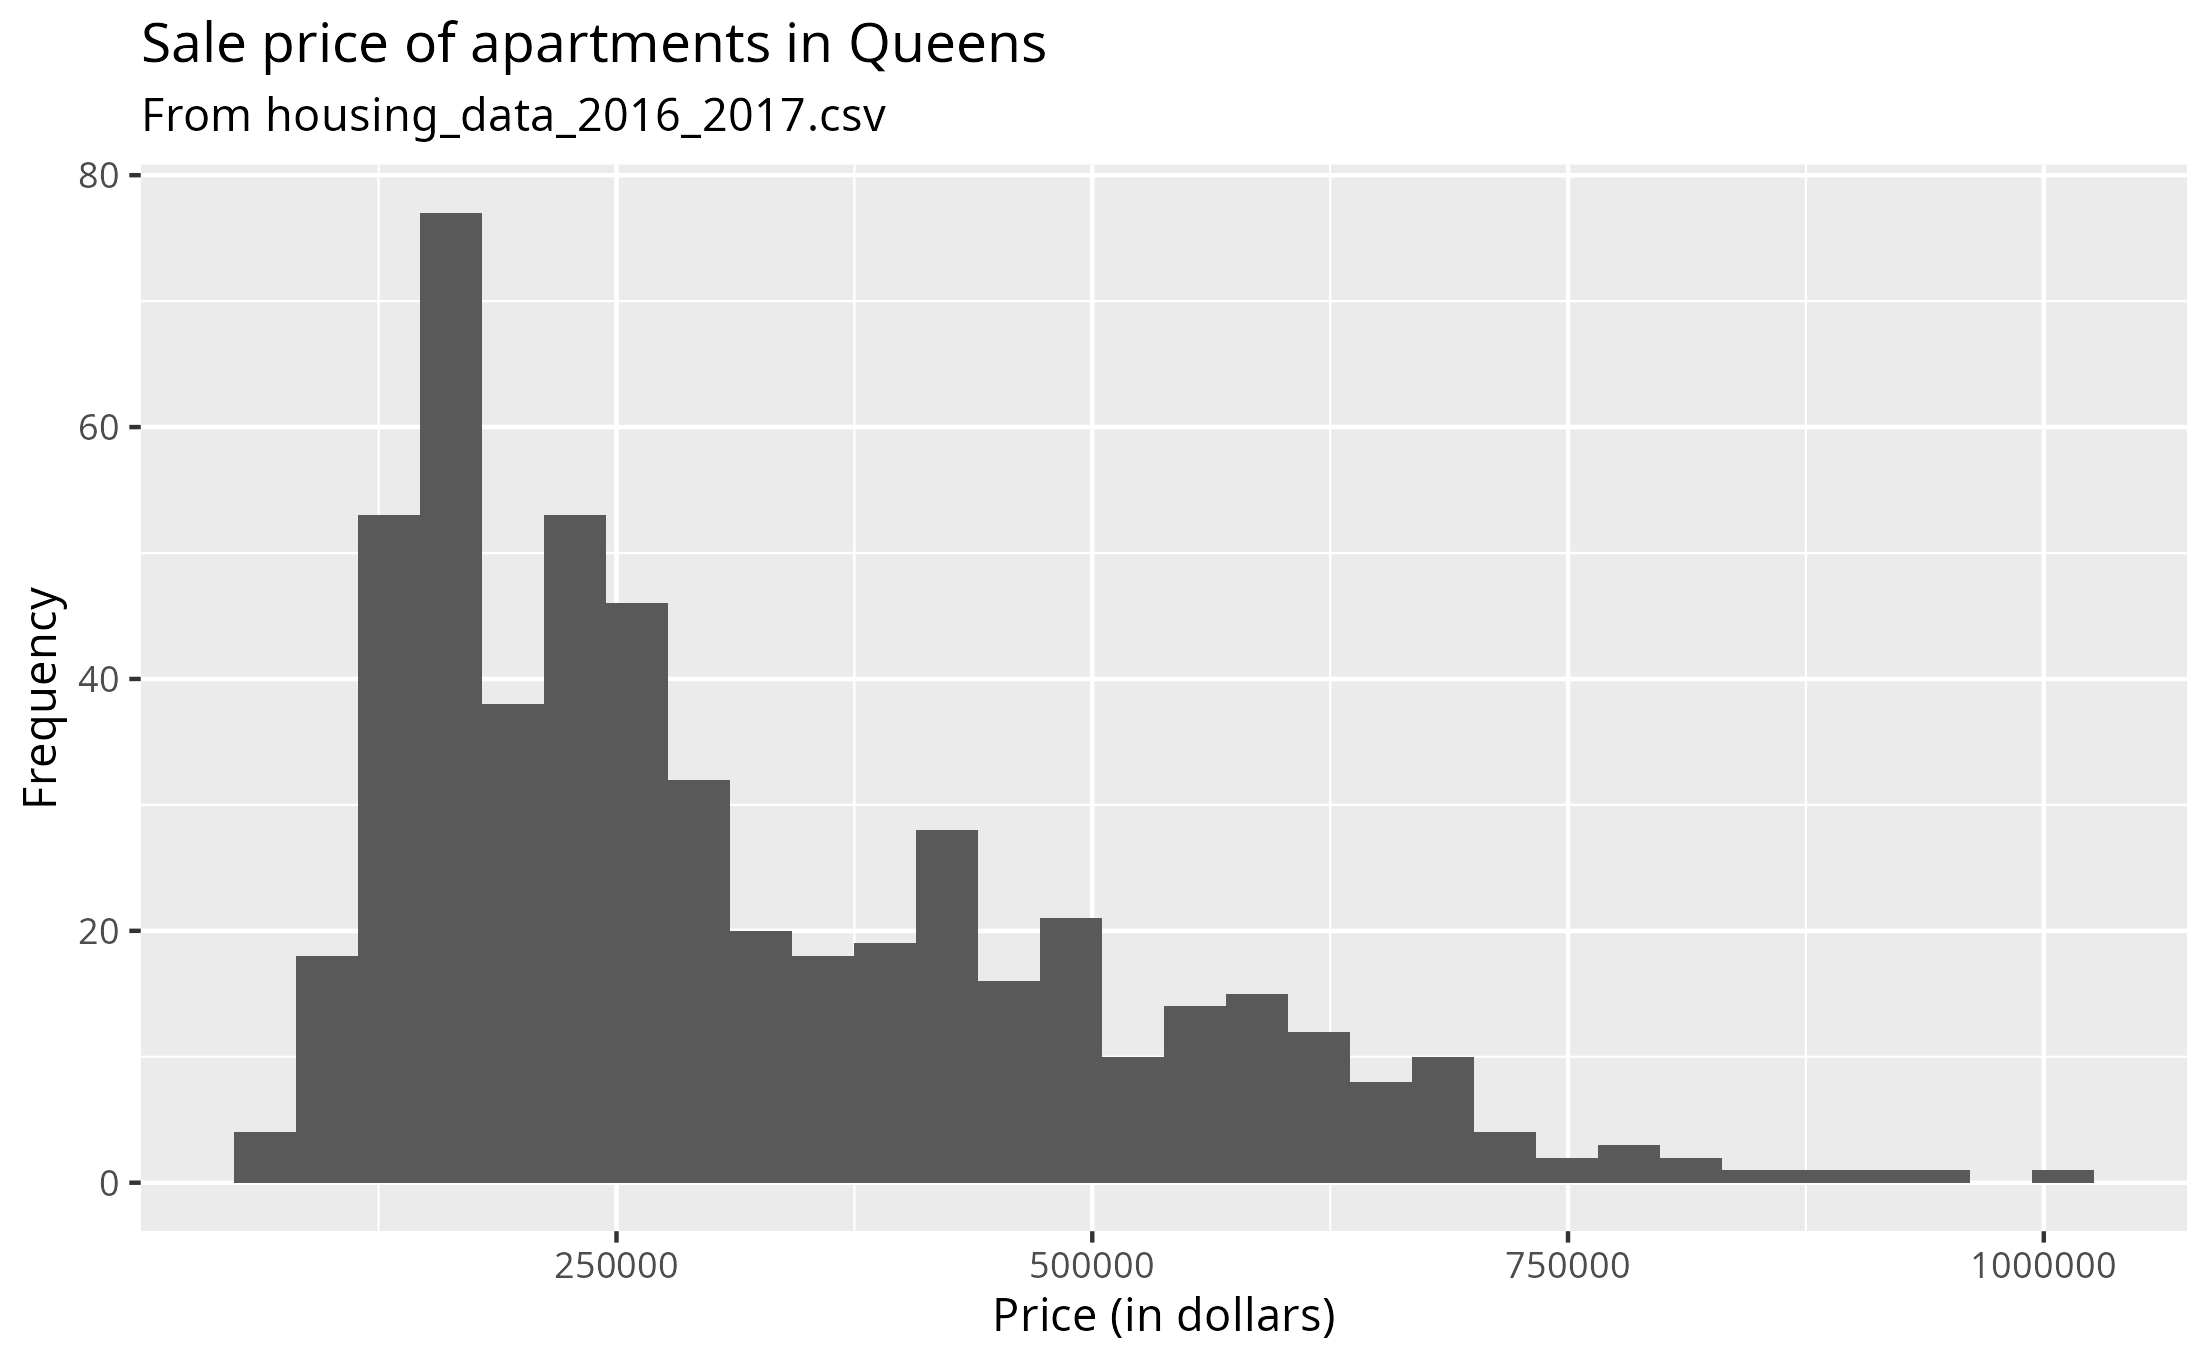
\includegraphics[width=0.7\textwidth]{apartment_sale_price_histogram.png}
		\label{fig:sale-price-hist}
		\caption{Histogram of sale prices for Queens apartments in the MLSLI data set.}
	\end{figure}
	Figure~\ref{fig:sale-price-hist} shows a histogram
	of the sale prices for the observations that list it. From this
	right-skewed data set, we may have potential outliers on the right-end
	with apartments priced at \$999,999. From this we expect the model predictions
	may be more accurate for apartments in the \$175,000-\$275,000 range.
	\subsection{Featurization}
	In my model I am using 21 features.
	Table~\ref{tbl:nominal-features} shows a summary of the nominal features.
	\begin{table}
		\footnotesize
		\begin{tabular}{|p{0.22\linewidth}|p{0.30\linewidth}|c|p{0.35\linewidth}|}
			\hline
			\textbf{Feature} & \textbf{Description} & \textbf{Missing Count} & \textbf{Percents}\\
			\hline
			
			\verb|cats_allowed| &  Whether cats are allowed in the apartment. & 0 & 
			\begin{center}
				\begin{tabular}{cc}
					\verb|No|: 62.87\% & \verb|Yes|: 37.13\%
				\end{tabular}
			\end{center}
			
			\\
			\hline
			\verb|community_district_num| & The number of the district in which
			an apartment is located. & 19 &
			\begin{center}
				\begin{tabular}{rr}
					\verb|24|: 8.59\% & \verb|25|: 27.86\%\\
					
					\verb|26|: 16.10\% &\verb|27|: 5.02\%\\
					
					\verb|28|: 26.37\% &\verb|29|: 3.08\%\\
					
					\verb|30|: 10.22\% &\textit{other}: 2.76\%
				\end{tabular}
			\end{center}
			\\
			
			\hline
			
			\verb|coop_condo| &  Whether an apartment is a co-op or a condo. & 0 & 
			\begin{center}
				\begin{tabular}{cc}
					\verb|co-op|: 74.48\% & \verb|condo|: 25.52\%
				\end{tabular}
			\end{center}
			\\
			
			\hline
			
			\verb|dining_room_type| & The type of dining room in the apartment. & 448 & 
			\begin{center}
				\begin{tabular}{rr}
					\verb|combo|: 53.70\% &\verb|formal|: 34.79\%\\
					
					\verb|none|: 0.11\% &\verb|other|: 11.39\%
				\end{tabular}
			\end{center}
			\\
			
			\hline
			
			\verb|dogs_allowed| & Whether dogs are allowed in the apartment. & 0 & 
			\begin{center}
				\begin{tabular}{cc}
					\verb|No|: 75.52\% &\verb|Yes|: 24.48\%
				\end{tabular}
			\end{center}
			\\
			
			\hline
			
			\verb|fuel_type|  & The type of fuel using for heating, including
			cooking. & 112 &
			\begin{center}
				\begin{tabular}{rr}
					\verb|electric|: 2.93\% & \verb|gas|: 63.64\%\\
					\verb|none|: 0.01\% &\verb|oil|: 31.35\%\\
					\verb|other|: 1.94\%
				\end{tabular}
			\end{center}\\
			
			
			\hline
			
			\verb|garage_exists| & Whether a garage is available at the premises. & 0 &
			\begin{center}
				\begin{tabular}{rr}
					\verb|No|: 81.88\% & \verb|Yes|: 18.12\%
				\end{tabular}
			\end{center}\\
			
			\hline
			
			\verb|kitchen_type| & The type of kitchen in the apartment. & 17 &
			\begin{center}
				\begin{tabular}{rr}
					\verb|combo|: 18.03\% & \verb|eatin|: 42.57\%\\
					\verb|efficiency|: 38.36\% & \verb|none|: 1.04\%
				\end{tabular}
			\end{center}\\
			
			\hline
			
			\verb|region| & The region in Queens that an apartment belongs to, according ot its ZIP code. & 0 & 
			\begin{center}
				\begin{tabular}{r}
					\verb|central_queens|: 5.43\% \\ \verb|jamaica|: 6.41\%\\
					\verb|north_queens|: 24.93\% \\ \verb|northeast_queens|: 8.03\%\\  \verb|northwest_queens|: 3.50\% \\ \verb|southeast_queens|: 6.77\% \\
					\verb|southwest_queens|: 9.19\% \\ \verb|west_central_queens|: 20.49\%\\
					\verb|west_queens|: 15.25\%
				\end{tabular}
			\end{center}
			\\
			
			\hline
		\end{tabular}
		\label{tbl:nominal-features}
		\caption{Summary of nominal features in data set.}
	\end{table}
	Table~\ref{tbl:continuous-features} shows a summary of the continuous
	features.
	\begin{table}
		\footnotesize
		\begin{tabular}{|p{0.22\linewidth}|p{0.30\linewidth}|c|c|c|c|c|}
			\hline
			\textbf{Feature} & \textbf{Description} & \textbf{Missing} & \textbf{Average} & \textbf{Std. Dev} & \textbf{Min} & \textbf{Max}\\
			\hline
			
			\verb|approx_year_built| & Approximate year when apartment was built. & 39 & 1963 & 21.1 & 1893 & 2017\\
			\hline
			
			\verb|num_bedrooms| & Number of bedrooms in apartment. & 115 & 1.65 & 0.744 & 0 & 6\\
			\hline
			
			\verb|num_floors_in_building| & Number of floors in the building of the apartment. & 650 & 7.79 & 7.52 & 1 & 34\\
			\hline
			
			\verb|num_full_bathrooms| & Number of full bathrooms in apartment. & 0 & 1.23 & 0.445 & 1 & 3\\
			\hline
			
			\verb|num_half_bathrooms| & Number of half bathrooms in apartment (no tub). & 2058 & 0.953 & 0.302 & 0 & 2\\
			\hline
			
			\verb|num_total_rooms| & Total number of rooms in apartment. & 2 & 4.14 & 1.35 & 0 & 14\\
			\hline
			
			\verb|parking_charges| & Charge for parking a vehicle in apartment premises. & 1671 & \$107.57 & \$70.88 & \$6.00 & \$837.00\\
			\hline
			
			\verb|pct_tax_deductibl| & Expense that can be subtracted from taxable income. & 1754 & 45.40\% & 6.95\% & 20.00\% & 75.00\%\\
			\hline
			
			\verb|sq_footage| & Amount of area (space) in apartment in square feet. & 1210 & 955 & 381 & 100 & 6215\\
			\hline
			
			\verb|total_taxes| & Total dollar amount paid in taxes. & 1646 & \$2,226.09 & \$1,850.09 & \$11.00 & \$9300.00\\
			\hline
			
			\verb|walk_score| & A measure of access to amenities by walking. & 0 & 83.9 & 14.8 & 7.00 & 99\\
			\hline
			
			\verb|monthly_charges| & Co-op or condo specific charges. & 193 & \$761.62 & \$395.87 & \$100.00 & \$4659.00\\
			\hline
		\end{tabular}
		\caption{Summary of continuous features.}
		\label{tbl:continuous-features}
	\end{table}
	From the nominal features, the \verb|region| was not initially available. To
	create it, I parsed the ZIP codes from the \verb|URL|, \verb|full_address_or_zip_code|,
	and \verb|url| columns in the raw data set. Then, I grouped
	the ZIP codes according to the region they belong to, dropping the three
	aforementioned columns thereafter. I did this with the intent
	of obtaining better interpretability, possibly at the expense of predictive power.
	Among the continuous features, I featurized \verb|monthly_charges| from the
	\verb|common_charges| and \verb|maintenance_cost| columns in the raw data set.
	The rationale is that these correspond to condos and co-ops, respectively,
	rather than accepting the missingness and imputing, it made sense to unify
	them into a single feature. The remaining columns were provided in the raw
	data, and some that do not appear, such as \verb|listing_price_to_nearest_1000|
	and \verb|date_of_sale|, were selected for dropping after judging them
	to be inappropriate predictors of the \verb|sale_price|.
	
	\subsection{Errors and Missingness}
	When I first loaded the data set into R, I looked at each column in turn
	to familiarize of myself with the values and get a sense for how much
	data was missing. Of the available data, there were many text input errors.
	The following are some examples:
	\begin{itemize}
		\item In the \verb|dogs_allowed| column, there were entries such as
		\verb|yes89| which were likely meant to be \verb|yes|.
		\item In the \verb|garage_exists| column, there were misspellings
		such as \verb|eys| and abbreviations such as \verb|UG| for \verb|underground|.
		\item In the \verb|kitchen_type| column, there were entries such as
		\verb|efficiemcy|, \verb|efficiency kitchene|, and
		 \verb|efficiency kitchen|. All of these were subsumed under
		 \verb|efficiency|.
	\end{itemize}
	For each such error, I either corrected to the value I presumed was correct,
	placed them into a pre-existing \verb|other| category, or set them as missing.
	I used regular expressions to streamline the detections and changes.
	
	The data set exhibited a lot of missingness as shown in Table~\ref{tbl:nominal-features}
	and Table~\ref{tbl:continuous-features}. In some cases, missingness resulted
	from certain patterns in the data. For example, \verb|common_charges|
	and \verb|maintenance_cost| were condo or co-op specific, respectively.
	Since there was no overlap between the columns (i.e., no row had a
	present value in both columns), I combined them according to the
	value of \verb|coop_condo| into a single column that retained their quantities.
	This condensing reduced missingness without needing to drop or manually
	alter the data. For \verb|garage_exists|, there were in fact 1826
	\verb|NA| entries, while all present entries had the value \verb|yes|.
	In this case, I decided to change all \verb|NA| entries to \verb|no|,
	making a possibly unjustified assumption about the respondent's original
	intent.
	
	The data set also exhibited missingness in the response column, \verb|sale_price|,
	with only 528 rows having a present value out of the total 2230. This meant that
	the model construction and validation could only rely on those 528 rows.
	However, rather than immediately discarding the rows for which \verb|sale_price|
	was missing, I retained them imputation. Before imputing, I split the 528 rows
	into $\mathbb{D}_{\text{train}}$, $\mathbb{D}_{\text{select}}$, and
	$\mathbb{D}_{\text{test}}$. I did this in anticipation of the need to perform
	model validation and hyperparameter selection. I set aside the response values
	in $\bm{y}_{\text{select}}$ and $\bm{y}_{\text{test}}$ into a copy, and then for the
	purposes of imputing, I temporarily set the responses in $\mathbb{D}_{\text{select}}$
	and $\mathbb{D}_{\text{test}}$ to missing (i.e. \verb|NA|), to ensure that they did
	not influence the imputed values, lest we risk having a dishonest model. For simplicity
	I did not include a matrix $M$ in the feature set that describes the missingness in
	the data set, which admittedly may have negatively affected performance of the
	trained models. To actually impute the values, I used the \textit{MissForest} algorithm
	as implemented by the \verb|missForest()| function in the \verb|missForest|
	package in R.
	\section{Modeling}
	\subsection{Regression Tree Modeling}
	The first candidate for a model I explored was a regression tree model.
	To compute the tree model, I used the \verb|YARFCART| function in the
	\verb|YARF| package. Since regression trees have a hyperparameter $N_0$
	for the threshold node size, I employed a hyperparameter selection procedure
	to select an optimal value for $N_0$. I tried 75 different node sizes, each an
	integer between 1 and 75, each time building a model on $\mathbb{D}_{\text{train}}$
	and computing the associated out-of-sample $RMSE$ by predicting on 
	$\mathbb{D}_{\text{select}}$. I chose the node size corresponding to the
	smallest out-of-sample error $RMSE$, which resulted in $N_0 = 23$.
	\begin{figure}
		\centering
		\makebox[0pt]{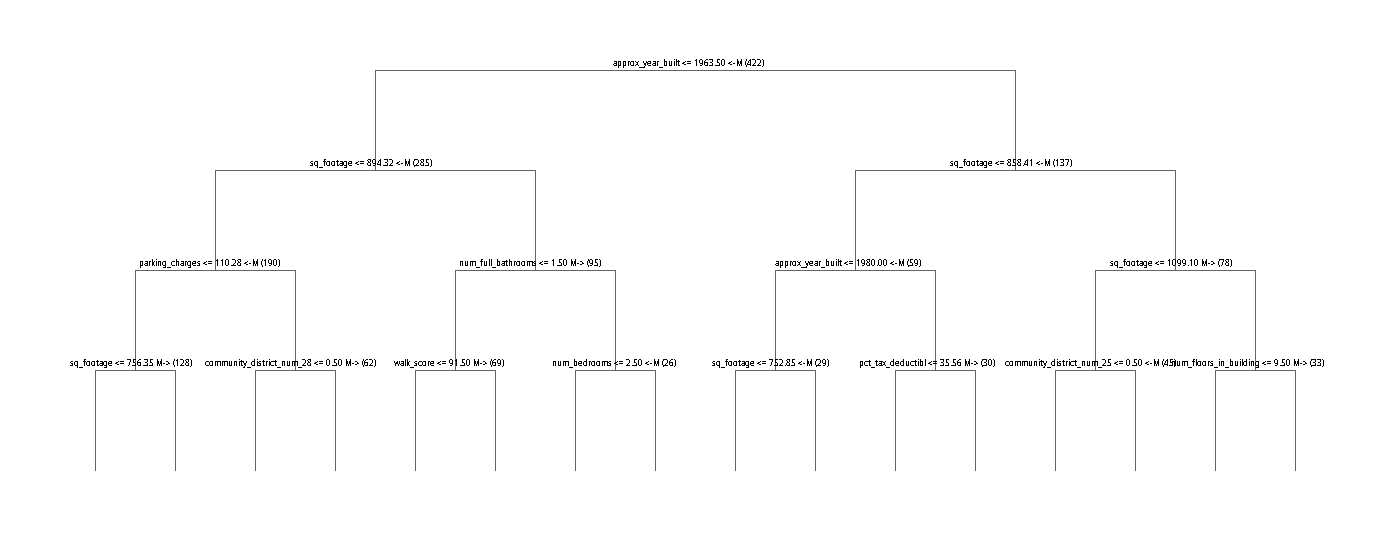
\includegraphics[width=1.4\linewidth]{tree_mod_report_1}}
		\caption{Top 4 layers in the regression tree model.}
		\label{fig:tree-mod-top-levels}
	\end{figure}
	Figure~\ref{fig:tree-mod-top-levels} illustrates the top 4 layers of the
	regression tree model. From the tree's top 5 layers (not depicted in that figure
	due to space), I determined the 10 most important features are:
	\begin{multicols}{3}
		\begin{itemize}
			\item \verb|approx_year_built|
			\item \verb|sq_footage|
			\item \verb|parking_charges|
			\item \verb|monthly_charges|
			\item \verb|total_taxes|
			\item \verb|pct_tax_deductible|
			\item \verb|num_floors_in_building|
			\item \verb|coop_condo|
			\item \verb|cats_allowed|
			\item \verb|community_district_number|
		\end{itemize}
	\end{multicols}
	The root split is according to whether the value of \verb|approx_year_built|
	is at most 1963, possibly suggesting that buyers care about how old a
	building is. The next most significant split appears to be whether
	\verb|sq_footage|, is around 800. It stands to reason that larger
	apartments tend to be more expensive. Though we can tell at a glance which are
	the most important features by inspecting the layers in the free,
	it's harder to discern their relative importance.
	\subsection{Linear Modeling}
	A line of best fit is a natural model to consider because of its simplicity.
	The advantage of a linear model is that its coefficients lend themselves
	to easy interpretations.
	
	\begin{table}
		\centering
		\small
		\begin{tabular}{|l|r|}
			\hline
			\textbf{Coefficient} & \textbf{Value}\\
			\hline
			Intercept	& -233675.88743	\\		
			\verb|approx_year_built|	& 99.20360\\
			\verb|cats_allowed1|&	2170.99809			\\
			\verb|community_district_num4|	& -107222.73430	\\
			\verb|community_district_num8| &	-109907.92626 \\
			\verb|community_district_num11| &	-49814.59426 \\
			\verb|community_district_num16|&	-98381.86284 \\			
			\verb|community_district_num19| & -45336.91857 \\
			\verb|community_district_num20| & -150148.56494 \\
			\verb|community_district_num23| &	-75037.36398 \\
			\verb|community_district_num24| &	-92355.11922 \\	
			\verb|community_district_num25| &	-16002.71146 \\		
			\verb|community_district_num26| &	-9545.76940	 \\	
			\verb|community_district_num27| &	-44494.12820 \\		
			\verb|community_district_num28| &	-58809.27350 \\		
			\verb|community_district_num29| &	-45284.99205 \\		
			\verb|community_district_num30| &	28255.00285	\\	
			\verb|coop_condocondo|	& 238345.93272 \\
			\verb|dining_room_typeformal|	& 11296.81763	\\
			\verb|dining_room_typeother|	& 17194.02611	\\
			\verb|dogs_allowed1| &	6835.33546			\\
			\verb|fuel_typegas| &	-8132.65876			\\
			\verb|fuel_typenone| &	16192.06722			\\
			\verb|fuel_typeoil| & 	2664.79414			\\
			\verb|fuel_typeother| &	-4278.77459			\\
			\verb|garage_exists1| &	16921.39471			\\
			\verb|kitchen_typeeatin| & -19453.39311	\\		
			\verb|kitchen_typeefficiency| & -38481.47712\\			
			\verb|num_bedrooms| & 37770.53423			\\
			\verb|num_floors_in_building| & 2338.81569	\\
			\verb|num_full_bathrooms| &	60791.15973			\\
			\verb|num_half_bathrooms| &	-9769.33225			\\
			\verb|num_total_rooms|	& 7516.83982			\\
			\verb|parking_charges|	& 444.93697			\\
			\verb|pct_tax_deductibl| & -2476.48258		\\	
			\verb|sq_footage|	& 14.85828			\\
			\verb|total_taxes|	& 14.09168			\\
			\verb|walk_score|	& 305.14194			\\
			\verb|regionjamaica| & -18065.91379	\\		
			\verb|regionnorth_queens| & 45578.83425	\\
			\verb|regionnortheast_queens| & 	42123.89355		\\	
			\verb|regionnorthwest_queens| & 	58988.52334		\\	
			\verb|regionsoutheast_queens| &	46595.00855		\\	
			\verb|regionsouthwest_queens| &	893.08745		\\	
			\verb|regionwest_central_queens| &	91744.35725	\\		
			\verb|regionwest_queens| &	55875.92791			\\
			\verb|monthly_charges| &	167.15893	\\
			\hline
		\end{tabular}
		\caption{Coefficients for linear model.}
		\label{tbl:coeffs-linear-mod}
	\end{table}
	Table~\ref{tbl:coeffs-linear-mod} shows the coefficients for
	the linear model computed. Consider, for example, the coefficient
	of \verb|approx_year_built|, which was deemed most important by
	the regression tree model. Its corresponding coefficient in
	the linear model is 99.20360, which means that an increase by 1 year
	results in around \$99.20 change in \verb|sale_price|. Meanwhile,
	a change in \verb|sq_footage| appears to only imply an increase by \$14.86
	in \verb|sale_price|. The largest coefficients in absolute value
	appear to be \verb|coop_condocondo|, where a flip implies a value change
	of about \$238,345.93, which may be because condos tend to be more
	expensive than co-ops. The coefficient \verb|community_district_num20|
	has the largest absolute negative value, implying that deciding to
	purchase an apartment in this neighborhood implies the \verb|sale_price|
	reduces by \$-150,148.56. The reduction may suggest that the district
	is generally undesirable as a place to live. These sorts of questions
	mirror how people normally think, weighing the consequence of a change
	in a particular characteristic.
	
	How well does the linear model really do? Let's consider that
	by looking at the in-sample performance metrics:
	\begin{align*}
		\text{in-sample-}RMSE &= 68649.9 \\
		\text{in-sample-} R^2  &= 0.8697797 
	\end{align*}
	Let's also consider the corresponding out-of-sample metrics:
	\begin{align*}
		\text{out-of-sample-}RMSE &= 80312.78\\
		\text{out-of-sample-} R^2 &= 0.801584 
	\end{align*}
	The increase in $RMSE$ and decrease in $R^2$ suggests the linear model
	is fitting some of the noise in the data. In spite of its seemingly
	impressive error metrics, the linear model fails to account for
	nonlinearities and interactions that surely exist in the data.
	Another issue is that linear models tend to extrapolate poorly.
	Indeed, this is the classic trade-off of interpretability and
	performance that we alluded to. These reasons make the linear model
	unsuitable for prediction.
	\subsection{Random Forest Modeling}
	In contrast with the linear model, the random forest model introduces
	the robustness necessary for complex interactions. Recall that
	the $RMSE$ metric is defined as $\sqrt{MSE}$, where $MSE$ is the
	Mean-Squared Error. In turn, the error accrued in the $MSE$ can
	be decomposed into bias and variance:
	\begin{align*}
		MSE := \text{Irreducible ignorance error} + \text{Bias} + \text{Variance}
	\end{align*}
	The random forest model is effective because it simultaneously reduces
	the bias and variance. It reduces the bias by using regression trees that
	are strong learners, i.e., trees with low bias yet high variance.
	To reduce variance, it uses two techniques: bootstrap aggregation
	and parameter subsetting.
	
	\begin{itemize}
		\item In bootstrap aggregation, we compute
		$M$ bootstrap samples, where for each time we sample with replacement
		out of the $n$ observations in the data set $\mathbb{D}$. Then,
		on these $M$ bootstrap samples $\mathbb{D}_1,\ldots,\mathbb{D}_M$,
		we compute corresponding tree models $g_1,\ldots,g_M$, and we compute
		their average $g_{\text{avg}} := \frac{1}{M}\sum_{m=1}^{M}g_m$. Each
		bootstrap has about two-thirds of the original data, and they all
		miss a slightly different one-third of the data. This results in the
		$M$ models $g_1,\ldots,g_M$ having loosely coupled, hence they
		have low covariance, and hence $g_{\text{avg}}$ has low variance.
		\item To take this a step further, random forest uses only a random subset of
		the features to build each tree model, and since the feature set
		used in each tree is slightly different, covariance further reduces.
	\end{itemize}
	Put together, these ensure the $MSE$ and hence the $RMSE$ is reduced.
	From the description, however, we see that there are a few hyperpameters
	that need to be set: the threshold node size $N_0$ as in regression trees,
	the number of trees (effectively $M$ as in the notation above), and the number
	$m_{\text{try}}$ of features for subsetting. To select appropriate values
	of these hyperparameters, I employed a hyperparameter selection procedure
	by creating a three-dimensional grid of values, where each value
	was a triplet $(m_{\text{try}}, M, N_0)$. I leveraged my $\mathbb{D}_{\text{select}}$
	and computed a random forest model for each triplet, in the end using
	the one that gave the lowest $RMSE$. The optimal hyperparameter values
	according to this procedure were:
	\begin{align*}
		m_{\text{try}} &= 19\\
		M &= 20\\
		N_0 &= 2
	\end{align*}
	The elaborate scheme described succeeds in improving performance, as
	can be seen from the out-of-sample performance metrics:
	\begin{align*}
		\text{out-of-sample-}RMSE &= 74097.86\\
		\text{out-of-sample-} R^2 &= 0.8311043 
	\end{align*}
	This is an improvement over the both the linear model and the
	single tree regression model. There is, however, some overfitting
	occurring, apparently more so than in the linear case:
	\begin{align*}
		\text{in-sample-}RMSE &= 34702.89\\
		\text{in-sample-}R^2 &= 0.9626422
	\end{align*}
	The overfitting may due to the relatively large number of features
	compared to the size of the data set. Moreover, although there
	was an improvement out-of-sample, we gained this at the expense
	of interpretability. Indeed, it is much harder to
	look at 20 different trees simultaneously, each using different features,
	and somehow understand how the model uses them to compute its prediction.
	Nevertheless, this model is the most flexible, is capable of accounting
	for complex interactions between the features, and generalizes well.
	
	\section{Performance Results}
	Table~\ref{tbl:oos-metrics-all-models} summarizes the performance of
	the three models we considered.
	\begin{table}
		\centering
		\begin{tabular}{|r|r|r|l|l|}
			\hline
			\textbf{Model} & $\mathbf{\textbf{in-sample-} RMSE}$ & $\mathbf{oosRMSE}$ &  $\mathbf{\textbf{in-sample-}R^2}$ &$\mathbf{oosR^2}$\\
			\hline
			Regression Tree Model & \$78,124.35 & \$101,784.00 & 0.8106687 & 0.6813115 \\
			\hline
			Linear Model & \$68,649.90  &\$80,312.78 & 0.8697797   & 0.801584\\
			\hline
			Random Forest Model & \$34,702.89 & \$74,097.86 & 0.9626422 & 0.8311043 \\
			\hline
		\end{tabular}
		\caption{Out-of-sample metrics for the three models we have considered.}
		\label{tbl:oos-metrics-all-models}
	\end{table}
	We see that the random forest beats the linear model by a small
	margin. The $R^2$ metric for all models is relatively close to $1$,
	implying that the proportion of variance explained is high.
	We can also say based on the out-of-sample $RMSE$ of the random forest
	model that the predictions will fall within \$148,195.72 (twice
	the $oosRMSE$) of the mean \verb|sale_price| \$314,956.60. This still
	quite a big range, and in fact it may not be useful enough for
	someone using the model to make an actionable decision related to
	an apartment purchase.
	
	The degradation in the error metrics is sharper in the tree and
	random forest models, suggesting that they are more prone to overfitting
	in this setting. The random forest model beats the linear model on the
	basis of its out-of-sample metrics. Moreover as we discussed earlier,
	it is likely to generalize better because it can handle interactions
	and nonlinearities in the data. However, due to the small sample size,
	and the fact that I did not do cross-validation, the out-of-sample
	metrics are not completely reliable.
	\section{Discussion}
	In this project, I compared the effectiveness of three different
	models in predicting apartment prices in Queens from 2016 to 2017.
	I familiarized myself with the data through data wrangling, cleaning,
	and employing missing data mechanisms. Working with the data enabled
	me to apply three predictive models that ranged in their simplicity,
	interpretability, and performance: a regression tree model, a linear
	model, and a random forest model. In the end, the random forest model
	was determined to be the most effective.
	
	In spite of these results, my approach was lacking in many areas.
	I made assumptions about features with a lot of missingness such
	as \verb|garage_exists| which may have had an unpredictable effect
	on the performance of my models. I also certain features such as
	the ZIP code into regions and possibly lost performance from it.
	I also noticed that some of my models suffered from not having
	all categories of certain features represented, and when going to
	predict out-of-sample, it resulted in these features ultimately
	being ignored, thereby biasing results (for example, community
	district number).
	
	Overall, I could have been more thoughtful in regards to feature
	engineering. To do a better job, I would work harder to understand
	the housing space and how the features interact. I would also
	search for ways to supplement the data set, with more observations
	and more features. To address the issue of representation, I
	would perform stratified sampling.
	
	Yet another area of improvement is in regards to error metrics.
	Since I did not perform cross-validation, the out-of-sample metrics
	are not very reliable in spite of being honest. As it stands,
	my random forest model is not production-ready, and it is not
	at the stage where it can beat a model curated by Zillow. However,
	by implementing some of the improvements suggested earlier,
	it may be able to improve enough to at least be useful.
	
	\pagebreak
	\section*{Code Appendix}
	\inputminted[bgcolor=LightGray]{r}{../final_project.Rmd}
	 
	%\pagebreak
	%\printbibliography
	
\end{document}
